\section{Goal Object}
Like many navigation algorithms, the one used in Chapter~\ref{ch:navigation}
requires the platform to have a goal location for which to traverse.
For these experiments, the goal location was provided to the robot by means
of a physical object that the robot could detect with its onboard camera.
The Nao API provides a simple ``red ball'' tracker that can be used to track
red objects via the onboard camera. It provides not only bearing information
but also range by assuming the red object has a width of $0.06 m$.

The goal was built as a $0.127 m$ wide red cube. 
This was affixed to the top of a wooden dowel, mounted to a heavy wooden base to 
allow it to be easily placed.
Figure~\ref{fig:red_cube1} shows a picture of the cube.
The dowel was approximately $0.6 m$ tall to allow the robot to see the cube
while minimizing the amount the head needs to pitch in order to keep 
the cube in view. Building the cube to be wider than the 
expected width allowed the target to be seen by the robot from longer distances. 
This longer range allowed for the construction of a larger arena as well as more 
robust tracking at shorter ranges.
The goal was built as a cube rather than a ball because during testing 
the tracking algorithm did not seem to be affected by the change in geometry 
and a cube was easier to construct. 

\begin{figure}
\centering
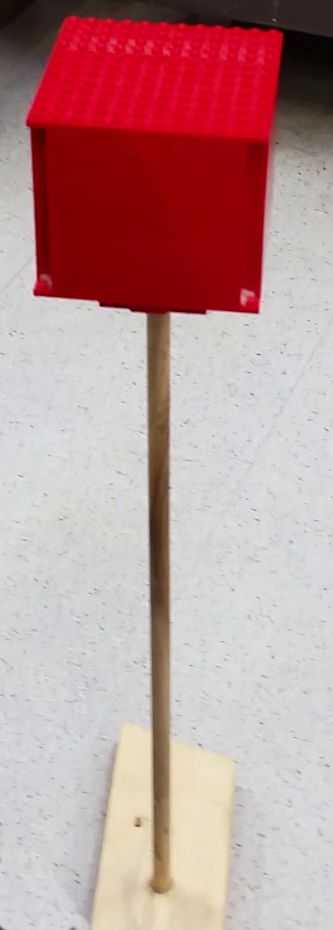
\includegraphics[height=0.4\textheight]{red_cube1.png}
\caption{Red cube that the Nao tracked as the goal location.}
\label{fig:red_cube1}
\end{figure}
